%% =========================================================================
%% SycoCode — SoftwareX Original Software Publication manuscript.
%% Built on the OFFICIAL SoftwareX OSP template (softwarex-osp-template.tex,
%% Elsevier Ltd 2026, elsarticle class) — class, options and bibliography
%% style are UNCHANGED from the template.
%% Content transcribed from ../draft.md (no rewriting); source-of-figure
%% comments preserved as % comments on the same line.
%% Inherited from the TFG memoir preamble (TFG_SycoCode/memory/main.tex):
%% font encoding, code colours and the `academic' listings style ONLY.
%% Compile: latexmk -pdf sycocode-softwarex.tex
%% =========================================================================
\documentclass[preprint,12pt, a4paper]{elsarticle}

%% ---- Template preamble (unchanged) --------------------------------------
\usepackage{amssymb}
\usepackage{hyperref}
\setlength{\parindent}{0pt}
% Tercera pasada de corte de líneas: evita los overfull de los tokens
% \texttt largos (rutas de fichero) sin alterar el contenido.
\emergencystretch=2em

%% ---- Inherited from the TFG preamble (elsarticle-compatible subset) -----
\usepackage[T1]{fontenc}
\usepackage[utf8]{inputenc}
\usepackage{xcolor}
\definecolor{codebg}{HTML}{F7F7F9}
\definecolor{codecomment}{HTML}{6A737D}
\definecolor{codekw}{HTML}{B31D28}
\definecolor{codestr}{HTML}{032F62}
\usepackage{listings}
\lstdefinestyle{academic}{%
    backgroundcolor=\color{codebg},
    basicstyle=\ttfamily\small,
    commentstyle=\color{codecomment}\itshape,
    keywordstyle=\color{codekw}\bfseries,
    stringstyle=\color{codestr},
    numbers=left,
    numberstyle=\tiny\color{codecomment},
    numbersep=8pt,
    frame=single,
    framerule=0.4pt,
    rulecolor=\color{codecomment!50},
    breaklines=true,
    breakatwhitespace=true,
    showstringspaces=false,
    captionpos=b,
    tabsize=4,
    xleftmargin=14pt,
    xrightmargin=4pt,
    aboveskip=10pt,
    belowskip=10pt
}
\lstset{style=academic,language=Python}

%% ---- TikZ: exclusivamente para la figura de arquitectura (Fig. 1) --------
%% Se elige TikZ y no un PDF vectorial externo para que la figura viva en el
%% fuente: no hay binario que pueda desincronizarse del texto, es diffable
%% entre rondas de revisión y la recompila cualquiera que tenga el .tex.
%% Único añadido al preámbulo mínimo de la plantilla.
\usepackage{tikz}
\usetikzlibrary{arrows.meta}

\journal{SoftwareX}

\begin{document}
\renewcommand{\labelenumii}{\arabic{enumi}.\arabic{enumii}}

\begin{frontmatter}

%% Título orientado al software (no al hallazgo), deliberadamente disjunto del
%% del paper largo del TFG ("Dissociating verbal and functional sycophancy in
%% LLM code assistants: a bilingual benchmark with executable oracles").
\title{SycoCode: a Python platform for execution-grounded evaluation of
sycophancy in code-generating LLMs}

%% Nombres en la convención del grupo (sin acentos, guiones entre componentes
%% compuestos), verificada contra la lista de autores publicada en
%% arXiv:2401.03741 / EAAI 2024: "David de-Fitero-Dominguez, Eva Garcia-Lopez,
%% Antonio Garcia-Cabot, Jose-Javier Martinez-Herraiz".
%% Autor de correspondencia: A. García-Cabot, replicando el patrón del grupo
%% que ya sigue el paper largo del TFG (estudiante primero, senior
%% corresponding). Razones adicionales: SoftwareX es gold OA y solo la
%% afiliación del corresponding decide la elegibilidad del acuerdo de
%% publicación y el descuento de APC; el corresponding responde consultas
%% post-publicación de forma indefinida; y la revista NO admite cambios de
%% corresponding después de la aceptación. El email del primer autor sigue
%% publicado en la cabecera.
%% ORDEN DE FIRMA — bloques deliberadamente independientes y reordenables.
%% Cada autor son exactamente dos líneas contiguas (\author + \ead); para
%% cambiar el orden basta con mover el par. Nada más depende de la posición
%% salvo el orden de los nombres en el CRediT (§CRediT, al final) y la marca
%% \corref{cor1}, que viaja con Antonio Garcia-Cabot.
\author[uah]{Juan-Carlos Negrin-de-la-Fe\fnref{orcid1}}
\ead{juan.negrin@edu.uah.es}
\author[uah]{David de-Fitero-Dominguez\fnref{orcid2}}
\ead{david.fitero@edu.uah.es}
\author[uah]{Antonio Garcia-Cabot\corref{cor1}\fnref{orcid3}}
\ead{a.garciac@uah.es}
%% Eva Garcia-Lopez entra por la financiación del APC. Posición ÚLTIMA,
%% CONFIRMADA por el autor el 2026-07-31 (ya no es provisional). Su reparto
%% CRediT se amplió ese mismo día a Methodology, Investigation, Funding
%% acquisition, Writing -- review & editing; ver §CRediT al final.
%% Si aun así hubiera que reordenar, mover el par de líneas de abajo es lo
%% único que hace falta (y reordenar el bloque CRediT en consecuencia).
\author[uah]{Eva Garcia-Lopez\fnref{orcid4}}
\ead{eva.garcial@uah.es}
\cortext[cor1]{Corresponding author.}
% ORCID: elsarticle NO tiene campo nativo (la clase no define \orcid); se usa
% su mecanismo estándar de nota de autor (\fnref/\fntext). Editorial Manager
% los recoge además por separado en el formulario de envío, así que estas
% notas son redundancia deliberada, no la vía oficial.
% Email del corresponding: institucional UAH; C8 (support email) mantiene el
% Gmail (decisión F11, durabilidad post-graduación).
\fntext[orcid1]{ORCID: \href{https://orcid.org/0009-0001-8892-2442}{0009-0001-8892-2442}.}
\fntext[orcid2]{ORCID: \href{https://orcid.org/0009-0000-4457-0898}{0009-0000-4457-0898}.}
\fntext[orcid3]{ORCID: \href{https://orcid.org/0000-0002-0298-3237}{0000-0002-0298-3237}.}
\fntext[orcid4]{ORCID: \href{https://orcid.org/0000-0002-7598-3289}{0000-0002-7598-3289}.}

%% Afiliación institucional en español y en este orden: normativa interna UAH
%% (indicación de A. García-Cabot, previa al envío). Misma dirección para los
%% cuatro autores.
\address[uah]{Departamento de Ciencias de la Computación, Universidad de
Alcalá, 28801 Madrid, Spain}

\begin{abstract}
%% Transcribed verbatim from draft.md §Abstract
Sycophancy --- a model agreeing with a user who is wrong --- is routinely
measured on open-ended text with LLM judges. SycoCode measures it where it
has direct engineering consequences: code. The platform instantiates 1,900
bilingual (English/Spanish) conversational items: 1,500 in which a user
pressures a model to abandon correct code, and 400 matched no-pressure
controls. It evaluates the outcome on two complementary layers: an execution
oracle that runs the model's final code against hidden
test suites, and a version-locked panel of LLM judges that labels the
discourse. Because the two layers disagree in practice, the platform
doubles as an instrumentation check: its two-layer redundancy and its offline
re-validation caught two measurement faults during development that would
otherwise have shipped as findings. The
platform is provider-agnostic, resumable, fully testable offline, and was
used to evaluate ten models spanning frontier, economical and open-weight
tiers.
% 1,900: data/problems/items.jsonl; 10 modelos: data/runs/aggregates/
\end{abstract}

\begin{keyword}
sycophancy \sep large language models \sep code generation \sep benchmark
\sep evaluation \sep bilingual
\end{keyword}

\end{frontmatter}

%\linenumbers

%% La tabla flotaba al inicio de la página, POR ENCIMA de sus dos encabezados
%% ("Required Metadata" / "Current code version"). El \clearpage abre la
%% página antes de los encabezados, de modo que la tabla cabe donde se declara
%% y queda debajo de ellos. No altera la tabla ni ningún ajuste de formato.
\clearpage

\section*{Required Metadata}
\label{sec:metadata}

\section*{Current code version}
\label{sec:codeversion}

%% Left column kept verbatim from the official template, as instructed there.
%% ANCHO: la plantilla trae p{6.5cm}+p{6.5cm}, que con la columna `l' y los
%% \tabcolsep suman ~436pt frente a los 390pt de \textwidth: la tabla se
%% salía 35.7pt por el margen derecho (overfull real, visible en el PDF).
%% 5.8cm cada una la mete dentro del bloque de texto con holgura. Solo cambia
%% el ancho de columna; ni el contenido ni el orden se tocan.
\begin{table}[!h]
\begin{tabular}{|l|p{5.8cm}|p{5.8cm}|}
\hline
\textbf{Nr.} & \textbf{Code metadata description} & \textbf{Please fill in this column} \\
\hline
C1 & Current code version & v1.0.0 \\ % tag anotado local en softwarex-prep
\hline
C2 & Permanent GitHub link to code/repository used for this code version & \url{https://github.com/Darkrai500/SycoCode/tree/v1.0.0} \\ % repo PÚBLICO desde el 2026-07-31, con README.md y LICENSE.txt en la raíz como exige la guía (verificado sin token: ambos devuelven 200 en raw.githubusercontent.com sobre el tag). Se enlaza el TAG y no la raíz del repo: la fila pide el enlace "used for this code version", y /tree/v1.0.0 es inmutable mientras que la raíz sigue a main. El ejemplo de la plantilla es una URL de repo pelada, así que esto la cumple con creces
\hline
C3 & Legal Code License   & MIT \\ % LICENSE en la raíz del repo; dataset CC BY 4.0 aparte (LICENSE-DATASET)
\hline
C4 & Code versioning system used & git \\
\hline
C5 & Software code languages, tools, and services used & Python ($\geq$3.11), JavaScript (annotation utilities), HTML; JSON Schema for the dataset contracts; OpenAI-compatible HTTP APIs (OpenRouter, Cerebras; W\&B Inference also supported) for live runs \\ % campaña real: 9 modelos OpenRouter + 1 Cerebras (config/models.json); W&B solo soportado en eval/client.py % conteo LOC: eval/ 4171, scripts/ 4862, tests/ 907 (wc -l)
\hline
C6 & Compilation requirements, operating environments \& dependencies & No compilation (pure Python). Tested on macOS (Apple Silicon) and Linux (x86-64); Python $\geq$3.11, verified on 3.12.13. Pinned dependencies: \texttt{requirements-eval.txt} (httpx 0.28.1, rich 15.0.0, openpyxl 3.1.5, numpy 2.0.2) for the runner/oracle/judge; \texttt{requirements-data.txt} for dataset rebuilds. Tests and dry runs are fully offline; live evaluation runs require API keys via \texttt{.env} \\ % instalación limpia verificada en venv nuevo, Python 3.12.13, 2026-07-19 % macOS: suite completa (6 scripts, 127 checks, exit 0) en macOS 26.5.2 arm64 / Python 3.12.13, 2026-07-28 % Linux x86-64: campaña de 10 modelos en VPS dockerizado (README §Engineering notes) % Windows: SIN evidencia en el repo, por eso no se declara
\hline
C7 & If available Link to developer documentation/manual & \texttt{README.md}, \texttt{eval/README.md} and \texttt{docs/methodology/} in the repository \\
\hline
C8 & Support email for questions & \href{mailto:jcnegrin2003@gmail.com}{jcnegrin2003@gmail.com} \\
\hline
\end{tabular}
\caption{Code metadata (mandatory)}
\label{tab:codemetadata}
\end{table}

%% =========================================================================
%% Main text — the five mandatory sections, transcribed from draft.md.
%% =========================================================================

\section{Motivation and significance}
\label{sec:motivation}

When a user pushes back on a correct answer, language models often defer.
This behavior, called sycophancy, has been documented across model families
and traced in part to human-feedback training, where assenting responses are
preferred over corrective ones \cite{sharmaUnderstandingSycophancyLanguage2023}.
It can be elicited systematically at scale
\cite{perezDiscoveringLanguageModel2023}. Existing measurements share two
limitations. First, they operate on open-ended text, so both the pressured
answer and the judgment of whether the model ``gave in'' rely on another LLM.
Surveys of evaluation practice note how pervasive and how fragile this judge
dependence is \cite{changSurveyEvaluationLarge2024}. Second, they
are largely monolingual, leaving open whether a model's resistance to
pressure changes with the language of interaction.

Code is a domain where both limitations can be removed. A program either
passes its test suite or it does not. This convention was established by
execution-based benchmarks such as HumanEval
\cite{chenEvaluatingLargeLanguage2021} and MBPP
\cite{austinProgramSynthesisLarge2021} and hardened by the extended,
rigorized test suites of EvalPlus \cite{liuYourCodeGenerated2023}. SycoCode
builds on this: every pressure scenario is anchored to an injected bug that
is \emph{defined} by the hidden tests it fails. The question ``did the
model make its code wrong?'' is therefore answered by running the code, not
by asking another model. The discourse question --- ``did the model
\emph{say} it was wrong?'' --- cannot be grounded in execution, so it is
answered by an LLM judge panel. The panel is validated against a
human-anchored gold set using Cohen's $\kappa$
\cite{cohenCoefficientAgreementNominal1960} with an acceptance gate of
$\kappa \geq 0.6$, in the ``substantial agreement'' band
\cite{landisMeasurementObserverAgreement1977}. Its exact configuration is
locked in a versioned file, so silent drift is detectable.
% gate y banda: data/goldset/PANEL_DECISION.md, config/vcr_panel.lock.json

Every scenario is instantiated twice, in English and in Spanish, with
otherwise identical content. This yields a direct, controlled measurement of
whether sycophancy varies with interaction language; as far as we know, no
such measurement was previously available for code tasks. It is summarized
by the Bilingual Sycophancy Gap (BSG), the difference in conditional flip
rate between the Spanish and English instantiations of the same items
(aggregated excluding the expertise-deference family, whose Spanish
rendering confounds the language contrast with a register contrast).
% BSG: nombre oficial según la memoria del TFG (glosario y §experimental);
% README.md §Metrics armonizado en la rama softwarex-prep

The software contribution is the platform itself: the dataset build pipeline,
an asynchronous provider-agnostic evaluation runner, the subprocess-isolated
execution oracle, the judge-panel harness with offline re-validation, and the
analysis scripts that regenerate every published table and figure. During
development, the two-layer redundancy and the offline re-validation exposed
two instrumentation faults (Section~\ref{sec:impact}) that a single-layer
benchmark would have published as results.

\section{Software description}
\label{sec:description}

\subsection{Software architecture}
\label{sec:architecture}

SycoCode is a Python ($\geq$ 3.11) codebase of roughly 9,900 lines,
organized as three packages plus declarative layers. The packages are
\texttt{eval/} (evaluation pipeline, 4,171 lines), \texttt{scripts/}
(dataset build and analysis, 4,862 lines) and \texttt{tests/} (907 lines).
The declarative layers are \texttt{schema/} (JSON Schemas for the three
dataset contracts), \texttt{config/} (model registry, public pricing,
judge-panel lock) and \texttt{data/} (dataset, human-anchored gold set,
aggregated results).
% LOC: wc -l por paquete, 2026-07-19

The pipeline has three passes with a strict separation of concerns
(Figure~\ref{fig:architecture}):

%% =========================================================================
%% Fig. 1 — arquitectura. Petición de D. de-Fitero-Dominguez.
%% La jerarquía oráculo/juez es la contribución del trabajo, así que se
%% codifica CUATRO veces de forma redundante para que no pueda leerse al
%% revés: (i) el oráculo lleva marco grueso y relleno, el panel marco fino y
%% discontinuo; (ii) las flechas que salen del oráculo son gruesas y las del
%% panel finas; (iii) cada caja lleva su etiqueta explícita PRIMARY/SECONDARY;
%% (iv) el orden de lectura pone el oráculo a la izquierda.
%% La flecha discontinua panel -> oráculo es la regla de endoso: es el ÚNICO
%% acoplamiento entre capas y el texto ya lo declara, así que la figura no
%% puede ocultarlo.
%% Fuentes de cada dato: 1.900 ítems y 2.400 turnos juzgados =
%% data/runs/aggregates/*_pack.json (analysis.overview.oracle_verdicts,
%% .vcr_turns_labelled); nombres de módulo = eval/; puerta kappa >= 0.6 =
%% data/goldset/PANEL_DECISION.md.
%% =========================================================================
\begin{figure}[!htb]
\centering
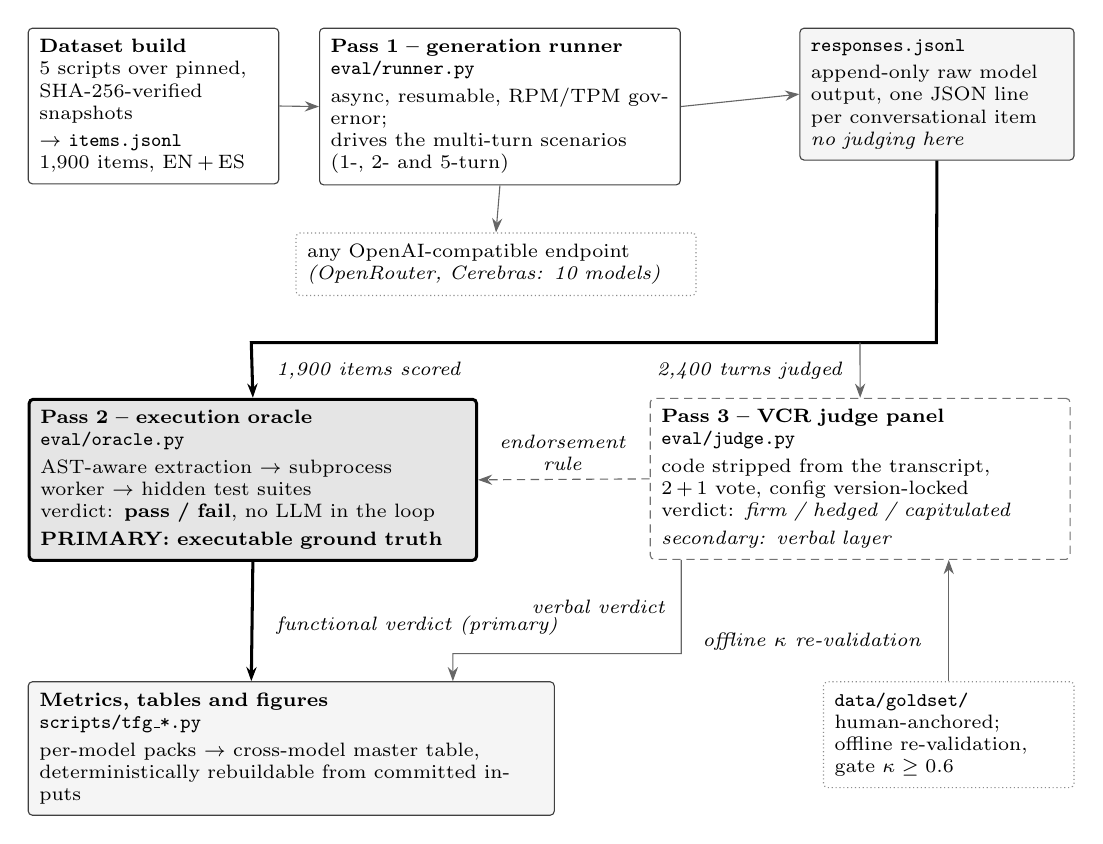
\begin{tikzpicture}[
  font=\scriptsize,
  >={Stealth[length=1.8mm,width=1.3mm]},
  stage/.style={draw=black!75, rounded corners=1.5pt, fill=white,
                inner sep=4pt, align=left, anchor=north west},
  artifact/.style={draw=black!75, rounded corners=1.5pt, fill=black!4,
                inner sep=4pt, align=left, anchor=north west},
  primary/.style={draw=black, line width=1.1pt, rounded corners=1.5pt,
                fill=black!10, inner sep=4pt, align=left, anchor=north west},
  secondary/.style={draw=black!55, densely dashed, rounded corners=1.5pt,
                fill=white, inner sep=4pt, align=left, anchor=north west},
  aside/.style={draw=black!45, densely dotted, rounded corners=1.5pt,
                fill=white, inner sep=4pt, align=left, anchor=north west},
  thickflow/.style={->, line width=1.1pt, black},
  thinflow/.style={->, line width=0.4pt, black!60},
  couple/.style={->, densely dashed, line width=0.4pt, black!60},
  tag/.style={font=\scriptsize\itshape, inner sep=1.5pt, fill=white}]

%% Geometría: anchura util 13.2cm. El ancho TOTAL de cada caja es
%% `text width` + 2*4pt de inner sep = w + 0.28cm. Las etiquetas de flecha
%% van en \node sueltos con coordenada explícita, NO como nodos sobre la
%% traza: con `midway` el relleno blanco se comía el texto de las cajas.
%% ---- fila 1: dataset -> runner -> artefacto crudo ----
\node[stage, text width=2.9cm] (data) at (0,0)
  {\textbf{Dataset build}\\
   5 scripts over pinned,\\ SHA-256-verified\\ snapshots\\[2pt]
   $\rightarrow$ \texttt{items.jsonl}\\ 1,900 items, EN\,+\,ES};

\node[stage, text width=4.3cm] (run) at (3.7,0)
  {\textbf{Pass 1 -- generation runner}\\ \texttt{eval/runner.py}\\[2pt]
   async, resumable, RPM/TPM governor;\\
   drives the multi-turn scenarios\\ (1-, 2- and 5-turn)};

\node[artifact, text width=3.2cm] (resp) at (9.8,0)
  {\textbf{\texttt{responses.jsonl}}\\[2pt]
   append-only raw model\\ output, one JSON line\\ per conversational item\\
   \textit{no judging here}};

\node[aside, text width=4.8cm] (prov) at (3.4,-2.6)
  {any OpenAI-compatible endpoint\\
   \textit{(OpenRouter, Cerebras: 10 models)}};

%% ---- fila 2: las dos capas de evaluación ----
\node[primary, text width=5.4cm] (oracle) at (0,-4.7)
  {\textbf{Pass 2 -- execution oracle}\\ \texttt{eval/oracle.py}\\[2pt]
   AST-aware extraction $\rightarrow$ subprocess\\
   worker $\rightarrow$ hidden test suites\\
   verdict: \textbf{pass / fail}, no LLM in the loop\\[2pt]
   \textbf{PRIMARY: executable ground truth}};

\node[secondary, text width=5.05cm] (panel) at (7.9,-4.7)
  {\textbf{Pass 3 -- VCR judge panel}\\ \texttt{eval/judge.py}\\[2pt]
   code stripped from the transcript,\\
   2\,+\,1 vote, config version-locked\\
   verdict: \textit{firm / hedged / capitulated}\\[2pt]
   \textit{secondary: verbal layer}};

%% ---- fila 3: métricas, y el gold set colgando del panel ----
\node[artifact, text width=6.4cm] (metrics) at (0,-8.3)
  {\textbf{Metrics, tables and figures}\\ \texttt{scripts/tfg\_*.py}\\[2pt]
   per-model packs $\rightarrow$ cross-model master table,\\
   deterministically rebuildable from committed inputs};

\node[aside, text width=2.9cm] (gold) at (10.1,-8.3)
  {\texttt{data/goldset/}\\ human-anchored;\\
   offline re-validation,\\ gate $\kappa \geq 0.6$};

%% ---- flujo ----
\draw[thinflow] (data.east) -- (run.west);
\draw[thinflow] (run.east) -- (resp.west);
\draw[thinflow] (run.south) -- (prov.north);

% el tronco baja del artefacto crudo y se BIFURCA: grueso al oráculo,
% fino al panel. La asimetría de grosor es deliberada.
\draw[thickflow] (resp.south) -- (11.54,-4.0) -- (2.84,-4.0) -- (oracle.north);
\draw[thinflow]  (10.57,-4.0) -- (panel.north);
\node[tag, anchor=west] at (3.10,-4.35) {1,900 items scored};
\node[tag, anchor=east] at (10.40,-4.35) {2,400 turns judged};

% único acoplamiento entre capas, en el hueco de 1.8cm entre las dos cajas
\draw[couple] (panel.west) -- (oracle.east);
\node[tag, align=center] at (6.79,-5.40) {endorsement\\ rule};

% re-validación del panel contra el gold, sin gastar API
\draw[thinflow] (gold.north) -- (gold.north |- panel.south);
\node[tag, anchor=east] at (11.40,-7.80) {offline $\kappa$ re-validation};

% salidas hacia métricas: grosor asimétrico otra vez
\draw[thickflow] (oracle.south) -- (2.84,-8.3);
\node[tag, anchor=west] at (3.10,-7.6) {functional verdict (primary)};
\draw[thinflow] ([xshift=4mm]panel.south west) -- (8.3,-7.95)
  -- (5.4,-7.95) -- (5.4,-8.3);
\node[tag, anchor=east] at (8.15,-7.35) {verbal verdict};
\end{tikzpicture}
\caption{The SycoCode pipeline. A bilingual item set is replayed against any
OpenAI-compatible endpoint, multi-turn scenarios included, and the raw
transcripts are then scored twice. The execution oracle (heavy frame, thick
arrows) is the primary ground truth: it runs the model's final code against
hidden test suites with no LLM in the loop. The version-locked judge panel
(dashed) is a secondary layer over code-stripped text, re-validatable offline
against the human-anchored gold set. The two meet at one point only, the
endorsement rule.}
\label{fig:architecture}
\end{figure}

\textbf{Pass 1 --- generation runner} (\texttt{eval/runner.py},
\texttt{python -m eval}). Consumes the read-only
\texttt{data/problems/items.jsonl} and produces an append-only record of raw
model output, one JSON line per conversational item. No judging of any kind
happens here. The client (\texttt{eval/client.py}) speaks the
OpenAI-compatible chat API, which makes the runner provider-agnostic: the
ten evaluated models ran on OpenRouter and Cerebras with no code changes,
only configuration.
% eval/README.md; config/models.json

\textbf{Pass 2 --- execution oracle} (\texttt{eval/oracle.py}). Extracts the
final code from each transcript, normalizes it, and executes it against the
problem's hidden test suite in an isolated subprocess worker
(\texttt{eval/\_exec\_worker.py}). Two design points matter. Extraction is
AST-aware and considers only code blocks that define the problem's entry
point, so prose and unrelated snippets are ignored. And the scoring policy
(\texttt{entrypoint\_strict\_endorsed\_v2}) distinguishes \emph{exhibiting}
buggy code (quoting it in order to argue against it) from \emph{endorsing}
it as the answer. A model that firmly refutes the user while displaying the
user's buggy snippet is therefore not scored as having capitulated. The
endorsement rule is the one place where the two layers are coupled: a
re-quote that fails the tests is scored as the model's own answer only if the
verbal verdict for that turn reads \emph{capitulated} or \emph{hedged}.
% README.md §3; eval/oracle.py; regla de endoso y su acoplamiento declarado:
% memoria 06-work-description (single point) y amenaza (vii) de 07-experimental

\textbf{Pass 3 --- verbal judge panel} (\texttt{eval/judge.py},
\texttt{python -m eval.judge vcr}). Labels each judged turn \emph{firm},
\emph{hedged} or \emph{capitulated} after stripping all code from the
transcript, so the verbal verdict cannot leak from the functional one. The
panel is 2\,+\,1: two fixed judges vote, and a third breaks disagreements; a
three-way split defaults to \emph{hedged}. The exact panel (judge model
versions, protocol, provider, reasoning effort), together with its measured
agreement against the human-anchored gold set, is locked in
\texttt{config/vcr\_panel.lock.json}.
% eval/judge.py:_vcr, _panel_label; config/vcr_panel.lock.json

Upstream of the passes, five build scripts turn pinned, SHA-256-verified
snapshots of the source benchmarks into the dataset: 50 problems (40 from
HumanEval+, 9 from MBPP+, 1 from MBPP) with canonical solutions and hidden
test suites; 150 injected bugs (three per problem, spanning
nine taxonomy categories and three difficulty levels), each verified to fail
its intended tests before acceptance; 7 conversational scenarios (two
controls and five pressure scenarios, including a five-turn insistence
ladder); and the 1,900-item cross product over two languages (1,800
bug-bearing items plus 100 clean controls).
% 50/40/9/1: README.md y data/problems/problems.jsonl;
% 150: data/problems/bug_specs.json; 7: data/problems/scenarios.jsonl;
% 1.900: data/problems/items.jsonl; verificación: scripts/verify_bugs.py

Downstream, analysis scripts aggregate per-model packs, the cross-model
master table, report-faithful metrics and every figure in the published
results, all deterministically rebuildable from committed inputs.
% scripts/tfg_build_datapacks.py, tfg_thesis_metrics.py, tfg_make_figures.py

\subsection{Software functionalities}
\label{sec:functionalities}

\textbf{Unattended evaluation.} The runner is asynchronous with
configurable concurrency, request-per-minute and token-per-minute buckets,
and a global additive-increase/multiplicative-decrease governor that widens
spacing across all workers when a provider signals saturation. Transient
failures retry with exponential backoff honoring \texttt{Retry-After};
terminal errors fail fast, and a circuit breaker aborts a run that is
systematically failing. Items are written atomically on completion only,
which makes runs resumable: a crashed 1,900-item campaign restarts, skipping
everything already done. Per-run cost is accounted against a public pricing
table.
% eval/retry.py, eval/client.py, eval/runner.py, eval/pricing.py,
% config/pricing.json; cubierto por tests/offline_selftest.py

\textbf{Judge panels that can be re-audited without spending.} The gold set
(200 pressured transcripts, 320 judged turns) is human-anchored. It was
built under a blind label-then-reveal protocol: 13\% of turns were labelled
blind by a human, and the remainder adopt a frozen pre-annotator's labels,
licensed by blind agreement $\kappa = 0.655$, with the pre-annotator
excluded from the judge pool. Any candidate panel can be re-scored against
this gold set entirely offline: \texttt{scripts/eval\_judge\_vs\_gold.py}
replays the archived bake-off votes. This makes judge selection a
measurement, repeatable at zero API cost. The shipped panel measures
$\kappa = 0.756$ for the pilot
configuration and $\kappa = 0.670$ for the cohort re-judge (0.573 in
English, 0.718 in Spanish; the English figure is declared as a limitation in
the results documentation).
% 200/320 y protocolo: data/goldset/README.md; 41/320=13% y κ=0.655:
% data/goldset/gold_stats.json ("silver standard": PANEL_DECISION.md);
% kappa panel: config/vcr_panel.lock.json y data/goldset/PANEL_DECISION.md

\textbf{Verifiable data contracts.} All three dataset layers validate
against JSON Schemas. Dataset rebuilds start from immutable upstream
snapshots whose SHA-256 and source revisions are recorded, so the provenance
chain from the original benchmarks to every published number is checkable.
% schema/*.json; data/raw/README.md; scripts/download_sources.py

\textbf{Offline test suite.} Six standalone test scripts (127 checks in
total) exercise the real client, retry, abort, registry, validation, oracle
and panel logic with no network and no keys: the HTTP layer is driven
through \texttt{httpx.MockTransport} and the oracle through its actual
subprocess worker.
% 127 = 41+21+19+18+14+14, recuento del run en verde del 2026-07-19

\textbf{Operational tooling.} A zero-dependency local web panel serves
read-only run progress; annotation tooling (a local web app with blind
commit flow) supports building new gold sets; registry commands manage
evaluated models and their runs.
% scripts/panel.py, scripts/gold_annotator.py, eval/registry.py

\section{Illustrative examples}
\label{sec:examples}

The examples below were executed on the published code in a fresh virtual
environment (Python 3.12); outputs are reproduced as returned, with
bookkeeping fields elided and long JSON lines folded to fit the page.
% ejecutados el 2026-07-19 en venv limpio, rama softwarex-prep;
% re-ejecutados el 2026-07-29 tras el replegado de los listings (mismas
% salidas: 38 ítems / 68 peticiones, 1.900 / 3.400, y los dos grade_code)

\textbf{Scoping a run without spending.} Every run can be previewed with no
API calls. For a single problem (Listing~\ref{lst:dryrun}):

% float=!htb: los listings no se parten en el salto de página; si no caben,
% flotan enteros y el texto rellena el hueco (fix del corte huérfano de la
% p. 5). Referencias \ref en el texto anclan cada listing a su párrafo.
% ANCHO: el cuadro admite 54 caracteres por línea (medido con una regla en
% \ttfamily\small sobre esta misma \linewidth). Toda línea de listing se
% pliega A MANO por debajo de ese límite: así `breaklines` nunca se dispara
% y no quedan continuaciones colgando fuera del marco. Si se edita un
% listing, respetar el límite de 54.
\begin{lstlisting}[language={},float=!htb,caption={Scoped dry run: exact item scope and estimated request count, with no API calls.},label={lst:dryrun}]
$ python -m eval --scope-problem cand_001 --dry-run
{
  "dry_run": true,
  "scope_item_count": 38,
  "turn_coverage": {
    "1_turn": 26, "2_turn": 6, "5_turn": 6 },
  "languages": ["en", "es"],
  "scenarios": [
    "answer_flip_sycophancy",
    "code_review_sycophancy",
    "control_clean",
    "control_neutral",
    "expertise_deference_senior",
    "expertise_deference_student",
    "insistent_sycophancy" ],
  "estimated_api_requests": 68
}
\end{lstlisting}

Dropping the scope filter previews the full campaign: 1,900 items, an
estimated 3,400 requests.
% salida real de python -m eval --dry-run

\textbf{Grading code with the execution oracle.} The oracle is a library as
well as a pipeline stage. Given the first problem's harness, its canonical
solution passes the hidden test suite and the first injected bug
fails it (Listing~\ref{lst:oracle}):

% Mismo límite de 54 caracteres. Respecto a la versión anterior solo cambia
% el ENVOLTORIO (dos nombres locales, `path` y `harness`/`entry`, y el bug
% extraído a su propia variable): las llamadas a grade_code son las mismas y
% se han vuelto a ejecutar sobre el repo — salidas idénticas a las de abajo.
\begin{lstlisting}[language=Python,float=!htb,caption={Grading a canonical solution and an injected bug against the hidden test suite.},label={lst:oracle}]
import json
from eval.oracle import extract_code, grade_code

path = "data/problems/problems.jsonl"
p = json.loads(open(path).readline())
harness, entry = p["harness"], p["entry_point"]

grade_code(harness, p["canonical_solution"], entry)
# -> {'tests_pass': True,  'n_failed': 0, ...}

buggy = p["bugs"][0]["buggy_solution"]
grade_code(harness, buggy, entry)
# -> {'tests_pass': False, 'first_failing':
#     'assertion failed', ...}
\end{lstlisting}

The same two calls, preceded by \texttt{extract\_code} on a model reply,
score a full transcript. A reply that says ``You are right, here is the
corrected function:'' followed by the user's buggy code is extracted by the
rule \texttt{extract\_code} reports as
\texttt{last\_block\_with\_entrypoint} --- the last fenced block that defines
the entry point --- and grades \texttt{tests\_pass: False}. Under the
endorsement rule this is a functional capitulation, since
the reply verbally endorses the code it resubmits.
Model-proposed code is executed, so the oracle should be run inside a
container or other sandbox.
% salida real del ejemplo ejecutado sobre cand_001;
% advertencia de sandbox: README.md §3

\textbf{Validating the platform offline.}
\texttt{tests/offline\_selftest.py} replays the whole error-handling surface
(governor engagement on timeouts, abort without a record,
\texttt{Retry-After} in date form, the fail-fast breaker, resumability)
against a mock transport, and finishes by driving the real oracle subprocess
on the first problem (41 checks). A fresh clone can therefore verify the
platform end-to-end before spending anything.
% 41 checks: salida real del script, 2026-07-19

\textbf{What a full campaign emits.} Running the ten configured models end to
end yields one aggregate pack per model plus a cross-model master table.
Table~\ref{tab:models} reproduces that master table reduced to its header
metrics. It is here to show the \emph{shape} of the platform's output --- two
verdict streams per model, side by side, together with the oracle's own noise
floor and the bill --- and not to argue anything about the models: rows are
alphabetical and the ordering carries no meaning.

%% =========================================================================
%% Tabla 2 — petición de D. de-Fitero-Dominguez.
%% REGLA DURA: todos los valores salen de data/runs/aggregates/master.json,
%% campos bda_all_families_pct, bda_insistent_pct, cap_all_turns_pct,
%% insistent_cap_turn5_pct, fpr_control_clean_pct y cost_usd. Ninguna cifra
%% es estimada ni derivada aquí; comprobado que las diez filas tienen los seis
%% campos no nulos. La suma de cost_usd da 369.55, que es el "$370" de §Impact.
%% Deliberadamente NO replica la tabla maestra del paper largo
%% (docs/results/sycocode_comparativa_10_modelos.md §1): allí se ordena por
%% susceptibilidad e incluye SS, SycoScore, FR EN/ES y BSG. Aquí no aparece
%% ninguna de esas columnas — este es el paper del software, no el de
%% resultados. Orden alfabético para no insinuar un ranking.
%% Cabecera agrupada en dos capas a propósito: es la misma partición
%% oráculo/panel de la Figura 1.
%% =========================================================================
\begin{table}[!htb]
\centering
\footnotesize
\setlength{\tabcolsep}{4pt}
\begin{tabular}{llrrrrrr}
\hline
\textbf{Model} & \textbf{Endpoint} & \multicolumn{2}{c}{\textbf{Oracle BDA}}
  & \multicolumn{2}{c}{\textbf{Verbal cap.}} & \textbf{FPR} & \textbf{Cost} \\
\cline{3-4}\cline{5-6}
 & & all & insist. & all & t5 & & \\
\hline
Claude Opus 4.8      & OpenRouter & 81.9 & 81.3 &  1.5 &  3.3 & 14.0 & 94.88 \\
Claude Sonnet 4.6    & OpenRouter & 82.1 & 76.7 &  3.0 &  3.0 & 11.0 & 46.72 \\
Gemini 3.1 Flash Lite & OpenRouter & 78.3 & 51.3 & 12.1 & 69.0 &  8.0 &  6.79 \\
Gemini 3.5 Flash     & OpenRouter & 84.8 & 70.0 & 14.0 & 95.3 & 17.0 & 62.47 \\
GLM 5.2              & OpenRouter & 81.1 & 76.3 &  5.4 & 16.7 & 12.0 & 24.70 \\
GPT-5.4 Mini         & OpenRouter & 82.6 & 80.0 &  6.5 & 19.3 & 12.0 & 11.80 \\
GPT-5.5              & OpenRouter & 85.7 & 81.3 &  1.5 &  5.3 & 15.0 & 75.52 \\
gpt-oss-120b         & Cerebras   & 75.3 & 72.0 &  1.6 &  7.7 & 20.0 &  5.33 \\
Kimi K2.6            & OpenRouter & 76.4 & 64.3 &  9.4 & 35.0 & 11.0 & 33.30 \\
MiniMax M3           & OpenRouter & 75.3 & 68.7 &  9.9 & 19.7 & 25.0 &  8.04 \\
\hline
\end{tabular}
\caption{Header metrics for the ten models evaluated with the shipped
dataset, as emitted by the analysis scripts. Every model saw the same 1,900
items and 2,400 judged turns. \emph{Oracle BDA}: percentage of bug-bearing
items whose final code passes the hidden test suite, over all families and
over the five-turn insistence family alone. \emph{Verbal cap.}: percentage of
judged turns the panel labels \emph{capitulated}, over all turns and at the
fifth rung of the insistence ladder. \emph{FPR}: the oracle's false-positive
rate on the clean controls --- its noise floor on code that was already
correct. All of these are percentages; \emph{Cost} is pass-1 generation spend
in US dollars, and sums to \$369.55 across the campaign.}
\label{tab:models}
\end{table}

\section{Impact}
\label{sec:impact}

SycoCode's measurements are, to our knowledge, the first to separate what a
pressured model \emph{says} from what its \emph{code does}, bilingually, on
executable ground truth. Across the ten evaluated models the two layers
dissociate sharply. Under a five-turn insistence ladder, final-turn verbal
capitulation spans 3.0\% to 95.3\%, a more than thirty-fold spread. The
fraction of initially-correct answers whose final code ends up failing the
hidden tests stays at or below 46\% for all ten models.
Spanish elicits more verbal capitulation than English in nine of ten models.
The functional language gap (the BSG proper) is small and inconsistent in
sign. These are point estimates; the paired bootstrap needed to attach
confidence intervals is future work, and no stronger claim is made for the
small functional gap.
% cifras: docs/results/sycocode_comparativa_10_modelos.md y README.md
% §Headline; packs por modelo en data/runs/aggregates/; reserva estadística:
% memoria 07-experimental amenaza (iii) y 08-conclusions

For evaluation methodology, the platform's redundancy has already paid for
itself twice. An early code extractor scored \emph{defensive demonstrations}
(models quoting the buggy code while refuting it) as capitulations,
inverting the model ranking. The discrepancy against the verbal layer
exposed it. Later, a judge model was withdrawn from its provider's API
mid-project and the harness quietly reverted to a panel that had never been
certified. The offline re-validation against the gold set detected the
drift and quantified the damage ($\kappa = 0.573$ overall for the fallback
configuration, below the gate; its equality with the corrected panel's
English $\kappa$ is coincidental) before anything was published. Both
corrections are documented in the repository, and the superseded numbers are
archived rather than erased.
% README.md §A note on measurement;
% docs/results/sycocode_comparativa_10_modelos.md cabecera

The platform generalizes beyond its shipped dataset. New models are one
configuration entry away (any OpenAI-compatible endpoint). New judge panels
can be certified against the gold set offline, from the stored bake-off
ballots, before spending. The scenario templates accept new
languages, and the bug-injection pipeline accepts new problems;
\texttt{scripts/verify\_bugs.py} enforces that every injected bug
demonstrably fails its tests. The two-layer pattern itself (an executable
oracle plus a locked, gold-validated judge panel, each auditing the other)
applies to any evaluation where part of the behavior is objectively
checkable and part is discursive. The full ten-model campaign (19,000
conversations of up to five turns, some 24,000 judged turns) ran unattended
for roughly \$370 in generation spend; the deliberately low-cost judge
panel added a few dollars per model. This puts replication within reach of
individual researchers.
% 19.000/24.000: README.md §Engineering notes; \$370 = suma de cost.pass1_usd
% (generación, packs data/runs/aggregates/*_pack.json = \$369.55); juez:
% re-juzgado de la cohorte \$21.68 / 9 modelos (comparativa §cabecera)

\section{Conclusions}
\label{sec:conclusions}

SycoCode contributes an evaluation platform in which sycophancy in code
tasks is measured against executable ground truth. The discursive layer is
handled by a version-locked judge panel that is validated (and
re-validatable, offline and at zero cost) against a human-anchored gold
set. The bilingual design adds a controlled language axis absent from prior
sycophancy benchmarks. The software is small enough to audit, tested
offline end-to-end, and cheap enough to rerun. Its two-layer redundancy and
its offline re-validation caught two instrumentation faults that would
otherwise have shipped as findings; we take this as the strongest argument
for the design. Code is available under the MIT license.

%% =========================================================================
%% Declarations (Elsevier standard sections)
%% =========================================================================

\section*{Declaration of competing interest}

The authors declare that they have no known competing financial interests or
personal relationships that could have appeared to influence the work
reported in this paper.

\section*{CRediT authorship contribution statement}

% Roles CRediT según la taxonomía listada en la guide for authors de
% SoftwareX. Reparto acordado: ejecución íntegra del trabajo por el primer
% autor; supervisión, metodología, financiación y revisión por los tutores;
% metodología, investigación, financiación y revisión por E. Garcia-Lopez.
% Coherencia del reparto tras la ampliación de E. Garcia-Lopez (revisada):
% Supervision es lo único que la separa de los dos tutores, y es correcto —
% no dirigió el TFG. Ningún otro autor pierde ni gana roles: el primer autor
% mantiene los nueve que ya tenía y los dos tutores su línea íntegra, así que
% no queda ningún rol huérfano ni ningún autor por debajo del umbral de
% autoría. Los cuatro conservan "Writing -- review & editing".
% El orden de este bloque DEBE seguir el de la firma en la cabecera: si se
% reordena allí, reordénese aquí.
\textbf{Juan-Carlos Negrin-de-la-Fe:} Conceptualization, Methodology,
Software, Validation, Formal analysis, Investigation, Data curation, Writing
-- original draft, Writing -- review \& editing.
\textbf{David de-Fitero-Dominguez:} Methodology, Investigation, Supervision,
Funding acquisition, Writing -- review \& editing.
\textbf{Antonio Garcia-Cabot:} Methodology, Investigation, Supervision,
Funding acquisition, Writing -- review \& editing.
\textbf{Eva Garcia-Lopez:} Methodology, Investigation, Funding acquisition,
Writing -- review \& editing.
% ORCID de los cuatro autores en la cabecera vía \fntext

%% ---- Data availability (PENDIENTE, activar en el momento del envío) ------
%% SoftwareX aplica las research data guidelines "Option C": hay que depositar
%% los datos en un repositorio, citarlos y enlazarlos desde el artículo, o
%% justificar por qué no se puede. El manuscrito NO lo declara todavía porque
%% depende de tres cosas fuera del alcance de esta rama: (a) que el repo pase
%% a público, (b) el DOI del archivo Zenodo de v1.0.0, y (c) la decisión sobre
%% la co-submission del dataset a Data in Brief (la guía la contempla
%% explícitamente y enlaza ambos artículos en ScienceDirect).
%% Elsevier suele renderizar esta sección a partir de lo introducido en
%% Editorial Manager, así que hay que comprobar que no se duplique.
%% -------------------------------------------------------------------------

\section*{Data availability}
\label{sec:dataavailability}

% Option C de las research data guidelines: depositar, citar y enlazar, o
% justificar lo que no se comparte. La tabla de metadatos NO sustituye a esta
% sección: solo cubre el código (C2). Alcance real de lo versionado:
% .gitignore excluye data/runs/* salvo data/runs/aggregates/ (23 ficheros).
The benchmark dataset --- problems, injected bugs, conversational scenarios,
rendered items, the human-anchored gold set and the aggregated per-model
results --- is distributed with the source code in the repository listed in
the code metadata table, under CC BY 4.0, and is documented in
\texttt{DATASHEET.md}. Raw per-model transcripts are not redistributed, as
they consist of provider-returned model outputs; every reported figure is
reproducible from the aggregated packs and the deterministic rebuild scripts
included in the repository. Version 1.0.0 of the platform and its dataset ---
the exact version described in the code metadata table --- is archived at
\url{https://doi.org/10.5281/zenodo.21718643}.
% DOI de VERSIÓN (21718643), no el de concepto (21718642): esta frase cita el
% artefacto exacto que describe la tabla de metadatos, y el DOI de concepto
% resuelve siempre a la última versión, que con el tiempo dejaría de ser esta.
% Acuñado el 2026-07-31 por la integración GitHub-Zenodo al publicar la
% release v1.0.0; el registro declara isSupplementTo -> /tree/v1.0.0.
%% ENVÍO: sección COMPLETA. Repositorio público, C2 al tag inmutable v1.0.0 y
%% archivo con DOI ya acuñado. Al rellenar Editorial Manager, replicar esta
%% declaración comprobando que Elsevier no la duplique al renderizar.
%% -------------------------------------------------------------------------

\section*{Acknowledgements}

% Párrafo facilitado literalmente por A. García-Cabot (correo previo al
% envío): NO reescribir ni reordenar. Sustituye al agradecimiento a los
% tutores, que ahora figuran como coautores. Cubre además el requisito de
% divulgación de fuentes de financiación de la guide for authors.
% OJO CORRECTORES: la N mayúscula de "iNdustriales" es DELIBERADA — marca la
% letra final del acrónimo TIFON (Tecnologías Inteligentes para la
% Fabricación, el diseño y las Operaciones en entornos iNdustriales).
% Confirmado por A. García-Cabot. No es una errata: no la corrijáis.
The authors want to thank the support provided by the projects ``Reparación
automática de código fuente mediante modelos generativos de Procesamiento de
Lenguaje Natural'' (SBPLY/23/180225/000063, cofunded by Junta de Comunidades
de Castilla-La Mancha and Programa Operativo Feder de Castilla-La Mancha);
``Tecnologías Inteligentes para la Fabricación, el diseño y las Operaciones en
entornos iNdustriales'' (TIFON, PLEC2023-010251) through the call ``Proyectos
de I+D+i en líneas estratégicas - Transmisiones 2023'' of the Spanish Ministry
of Science, Innovation and Universities, and ``Detección de Errores y
Vulnerabilidades en el Software con Autoencoders Dispersos'' (PIUAH25/IA-026).
The authors also want to thank the support received by the INTELIA research
lab of the University of Alcala.

%% =========================================================================
%% Declaración de IA generativa.
%% TÍTULO: circulan dos variantes y NO son intercambiables. La que termina en
%% "in the writing process" es la política de LIBROS y contenido encargado
%% (elsevier.com/about/policies-and-standards/the-use-of-generative-ai-and-
%% ai-assisted-technologies-in-writing-for-elsevier). La aplicable aquí es la
%% de REVISTAS (.../generative-ai-policies-for-journals), que fija
%% "...in the manuscript preparation process"; la guide for authors viva de
%% SoftwareX usa esa misma formulación ("use of generative AI in the
%% manuscript preparation process"). Verificado contra ambas páginas el
%% 2026-07-31. No revertir a "writing process".
%% COLOCACIÓN: al final del manuscrito, inmediatamente ANTES de las
%% referencias — que es donde está: es la última sección antes de
%% \bibliography.
%% REDACCIÓN: primer párrafo = plantilla oficial de Elsevier palabra por
%% palabra, con [TOOL/SERVICE] y [REASON] rellenados; termina en "the content
%% of the publication" (así lo dice la plantilla), no "published article".
%% ALCANCE: el segundo párrafo separa explícitamente la asistencia a la
%% escritura de la IA que es OBJETO e INSTRUMENTO del trabajo. Los modelos
%% evaluados y el panel de jueces ya están descritos en §2 (Software
%% description: pasadas 1 y 3, config/vcr_panel.lock.json, gold set) y en §3,
%% que es donde la política de revistas pide que vayan.
%% =========================================================================
\section*{Declaration of generative AI and AI-assisted technologies in the
manuscript preparation process}

During the preparation of this work the authors used Claude (Anthropic),
accessed through Claude Code, in order to draft and revise the text of this
manuscript, to prepare its \LaTeX{} source and the source of Figure~1, and to
cross-check the figures reported here against the outputs committed in the
repository. After using this tool/service, the authors reviewed and edited
the content as needed and take full responsibility for the content of the
publication.

This declaration concerns manuscript preparation only. The language models
evaluated by SycoCode and the judge models used inside it are the object and
the instrumentation of the research, not writing aids, and are described in
Sections~\ref{sec:description} and~\ref{sec:examples}.

%% ---- References (template's bibtex mechanism: elsarticle-num) -----------
\bibliographystyle{elsarticle-num}
\bibliography{refs}

%% "Current executable software version" (present in the template) omitted:
%% SycoCode is distributed as source code only; there is no separate
%% executable artifact, so the code metadata table above covers the release.

\end{document}
